% Metódy inžinierskej práce

\documentclass[10pt,twoside,slovak,a4paper]{article}

\usepackage[slovak]{babel}
%\usepackage[T1]{fontenc}
\usepackage[IL2]{fontenc} % lepšia sadzba písmena Ľ než v T1
\usepackage[utf8]{inputenc}
\usepackage{graphicx}
\usepackage{url} % príkaz \url na formátovanie URL
\usepackage{hyperref} % odkazy v texte budú aktívne (pri niektorých triedach dokumentov spôsobuje posun textu)

\usepackage{cite}
%\usepackage{times}

\pagestyle{headings}

\title{Budúcnosť školských tried\thanks{Semestrálny projekt v predmete Metódy inžinierskej práce, ak. rok 2020/21, vedenie: Ing. Fedor Lehocki, PhD.}} % meno a priezvisko vyučujúceho na cvičeniach

\author{Marek Sunega\\[2pt]
	{\small Slovenská technická univerzita v Bratislave}\\
	{\small Fakulta informatiky a informačných technológií}\\
	{\small \texttt{xsunegam@stuba.sk}}
	}

\date{\small 30. september 2015} % upravte



\begin{document}

\maketitle

\begin{abstract}
	Táto štúdia nabádza k tomu, že virtuálne učebne nedosiahli svoj plný potencial. V článku sa 
	uvádza ako by mohla vypadať virtuálna trieda vzhľadom na špecifika výučby počas 
	prebiehajúcej pandémie COVID 19. Zisťuje výhody a nevýhody a odprezentuváva ich. Zameriava 
	sa na rôzne typy virtuálnych tried a ich diferencie. Ukazuje hlavné rozdiely medzi tradičnou 
	a virtuálnou výučbou a porovnáva ich efektívnosť. Či by to niečo znamenalo pre klasické vyučovanie 
	a ako veľmi by sa dala virtuálna výučba automatizovať. Dala by sa virtuálna výučba ešte viac 
	využívať ako dnes a ci má nejakú budúcnosť. Uvádza výhody a vplyvy na učiteľov, žiakov, na ich 
	výsledky a efektivitu učenia.
\end{abstract}



\section{Úvod}




\section{Nejaká časť} \label{nejaka}

Z obr.~\ref{f:rozhod} je všetko jasné. 

\begin{figure*}[tbh]
\centering
%\includegraphics[scale=1.0]{diagram.pdf}
Aj text môže byť prezentovaný ako obrázok. Stane sa z neho označný plávajúci objekt. Po vytvorení diagramu zrušte znak \texttt{\%} pred príkazom \verb|\includegraphics| označte tento riadok ako komentár (tiež pomocou znaku \texttt{\%}).
\caption{Rozhodujúci argument.}
\end{figure*}



\section{Skúsenosti z používania virtuálnych učební} \label{3}

Pre lepšie predstavenie autorových skúseností z dvadsiatich rokov používania virtuálnych učební 
v terciárnom vzdelávaní sú funkcie, dostupné vo väčšine prostredí virtuálnych učební, rozdelené do 
dvoch skupín. Do prvej skupiny (bežné funkcie) patria funkcie súvisiace iba s emuláciou tradičnej triedy. 
Druhá skupina (pokročilé funkcie) sa skladá z funkcií a postupov presahujúcich tradičné učebne. 
Tabuľka obsahuje obe kategórie.\cite{VCf}

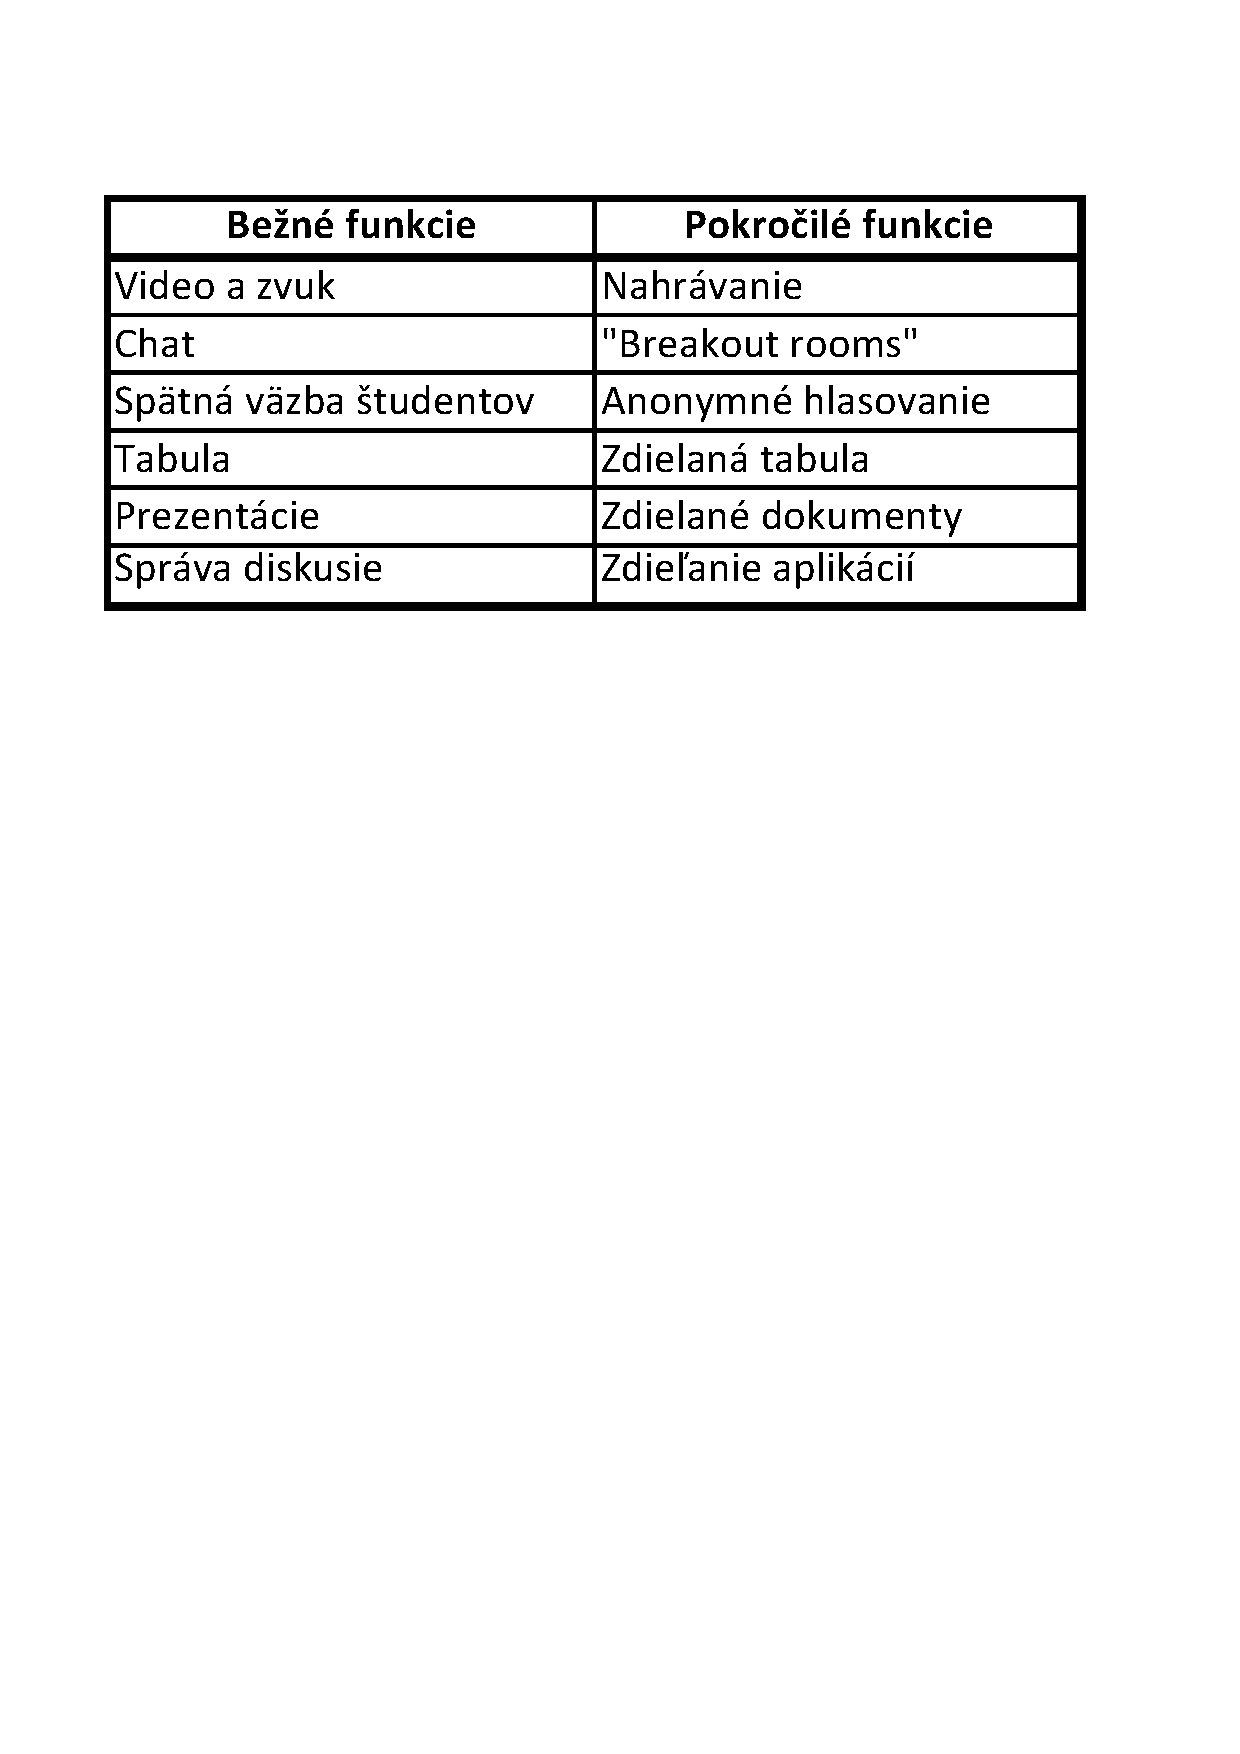
\includegraphics[scale=0.5]{tab1.pdf}\label{tab1}



\subsection{Bežné funkcie pre napodobnenie klasickej triedy} \label{Bezne}

\begin{itemize}
\item V súčasnosti je \textbf{video a zvuk} k dispozícii pre profesora aj študentov. Osvedčeným postupom je pokúsiť sa,
aby sa všetci študenti prezentovali na videu, najmä v prípadoch, keď sa nestretli zoči-voči. Je pravda,
že pri dištančnom vzdelávaní je stretnutie študentov aspoň raz cenený pre budovanie komunity a v prípadoch,
keď to nie je možné, je nevyhnutné predstaviť sa pomocou videa a zvuku.\cite{VCf}

	\item Funkcia \textbf{četu} môže vždy pomôcť prekonať problémy so zvukom, a hoci nesúvisí s tradičnou praxou v triede, 
je uvedená v tomto zozname aj z historických, aj praktických dôvodov.Funkcia četu by okrem riešenia zvukových problémov 
mohla študentom umožniť lepšie objasniť otázku alebo umožniť profesorovi zbierať krátke odpovede, najmä ak chat podporuje 
priame správy medzi študentom a učiteľom, ako to robí väčšina súčasných virtualnych prostredí.\cite{VCf}

	\item \textbf{Správa diskusií} uľahčuje najnáročnejšiu úlohu,s ktoroú sa musí profesor vo virtuálnej učebne potrápiť.
Ovládanie publika s sledovanie „zdvihnutých rúk“  je niečo, čo si človek musí osvojiť v praxi.\cite{VCf}
\end{itemize}

\subsection{Pokročilé funkcie presahujúce tradičné učebne} \label{Pokr}
\begin{itemize}
	\item retrospective assignments
\end{itemize}	
\paragraph{Veľmi dôležitá poznámka.}
Niekedy je potrebné nadpisom označiť odsek. Text pokračuje hneď za nadpisom.



\section{Dôležitá časť} \label{dolezita}




\section{Ešte dôležitejšia časť} \label{dolezitejsia}




\section{Záver} \label{zaver} % prípadne iný variant názvu



%\acknowledgement{Ak niekomu chcete poďakovať\ldots}


% týmto sa generuje zoznam literatúry z obsahu súboru literatura.bib podľa toho, na čo sa v článku odkazujete
\bibliography{lit}
\bibliographystyle{plain} % prípadne alpha, abbrv alebo hociktorý iný
\end{document}
